\section{Trigger}
\label{sec:lhcb:trig}

With a $pp$ interaction rate of $40\mhz$ and multiple subdetector stations, there is too much
information associated with each event to write everything all to disk.
Instead a multistage trigger is employed to filter potentially interesting events based on track
momentum and energy.
The \lone is embedded in the hardware of \lhcb and is fully synchronous with
the bunch crossing rate, it reduces the output $1\mhz$.
There are five \lone trigger lines; one each for objects identified as
photons, electrons, hadrons, muons and pairs of muons (dimuon).
Two software triggers follow \lone, and are fast enough to perform tracking algorithms and use
information from
multiple subdetectors to reduce the events written to disk to $5\khz$.
The flow of data through the trigger is shown in Fig.~\ref{fig:lhcb:trigger}.

\begin{figure}
  \begin{center}
    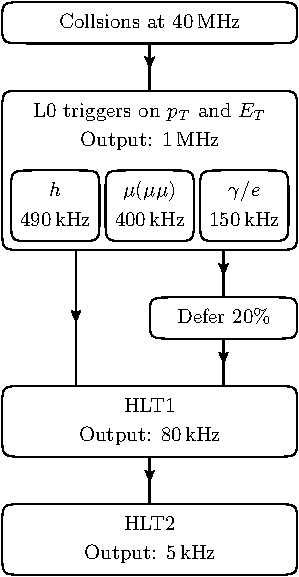
\includegraphics[scale=1]{trigger}
  \end{center}
  \caption[LHCb trigger sequence in 2012]
  {
    The flow of the \lhcb trigger system in 2012.
  }
  \label{fig:lhcb:trigger}
\end{figure}

%\lone trigger lines that accept events with muons use information from the muon system, while all
%others rely on calorimeter information.
The \lone trigger algorithms for photons, hadrons, and electrons are based on calorimeter objects.
A single calorimeter cluster is defined as two-by-two calorimeter cells in each the \ecal and
\hcal.
For each cluster the transverse energy, $E_T$, is calculated:
\begin{equation}
  E_T = \sum_{i=1}^4E_i\sin\theta_i,
\end{equation}
where $E_i$ is the energy in cell $i$ and $\theta_i$ is the angle between the average
interaction point and the cell's centre.
Clusters are categorized as follows.
A hadron candidate is the largest $E_T$ cluster in the \hcal summed with the $E_T$ of the \ecal
cluster in front, if there is one.
A candidate photon (electron) is the largest $E_T$ deposit with hits in the \presh cells in front and
no hits (at least one hit) in the nearest \spd cells.
The $E_T$ of each candidate is compared to thresholds, and the event is retained if one or more is
exceeded.

\lone trigger lines associated with muons base their acceptance on measurements of \pt.
Each quadrant of the muon system is read out independently, so muons which cross boundaries cannot
be triggered.
Muon candidates with the highest and second highest \pt are selected from each quadrant by
searching for straight lines through M1-5 in the \plane{z}{y}, and in the \plane{z}{x} if
$p_T>0.5\gev$.
The M1 station is used to increase the \pt resolution of muon tracks in the trigger without
tracking information: this achieves a resolution of about $25\,\%$ that of fully reconstructed
tracks.
Events are accepted based on candidates from all quadrants with values of $p_T^\mathrm{max}$ and
$p_T^\mathrm{max}\times p_T^\mathrm{2^{nd} max}$ greater than thresholds for the muon and dimuon
lines respectively.
Thresholds for \lone trigger lines used in this thesis are given in \Tab{tab:lhcb:trigger}.

\begin{table}
  \caption[Level one trigger thresholds]
  {
    Thresholds in 2011 and 2012 for \lone trigger lines~\cite{Albrecht:2013fba} used in this thesis.
  }
  \label{tab:lhcb:trigger}
  \begin{center}
    \begin{tabular}{ccc}\toprule
      &2011&2012\\\midrule
      {\tt L0Muon} & $1.48\gev$ & $1.76\gev$ \\
      {\tt L0Dimuon} & $(1.296\gev)^2$ & $(1.6\gev)^2$ \\
      {\tt L0Hadron} & $3.5\gev$ & $3.7\gev$ \\
      \bottomrule
    \end{tabular}
  \end{center}
\end{table}

Deferred triggering was introduced in 2012.
It diverts around $20\pc$ of events that pass the \lone trigger to hard disks for processing when
the \lhc is not colliding protons.
The $80\%$ of events accepted at are processed immediately by the software triggers, which are run
on around 2000 computing nodes using \cpp applications.

Following \lone, there are software \glspl{HLTLabel}.
The first software trigger, \hltone, performs the full three dimensional \velo track fitting
algorithms (but with fewer passes than the offline version).
Candidate \velo tracks for triggers which do not require muons are selected based upon the quality of the
\velo track and the smallest IP with respect to any of the identified primary vertices.
Primary vertices are defined to be points within $300\mum$ of the mean
interaction point in the \plane{x}{y}, $\mathrm{PV}^\mathrm{mean}_{xy}$, from which at least five
tracks originate.
The position of $\mathrm{PV}^\mathrm{mean}_{xy}$ is measured at the start of each \lhc machine
fill.
For trigger lines requiring muons, each \velo track is extrapolated to a window in the M3
station.
The size of this window is narrow in the non-bending direction but wide enough to accommodate a $6\gev$
muon in $x$.
If there is a deposit in this window then the \velo track, is extrapolated to the cluster and if
there are hits consistent with this track in any of the muon stations M2, M4 or M5 the track is
tagged as belonging to a muon.
The \velo tracks that are selected by IP or the muon system are extrapolated (or interpolated) into
the \intr and \ot.
This is known as forward tracking, and provides momentum measurements for all these tracks.

%More info needed on specific lines?

The \hltone output rate of $80\khz$ is sufficiently low to allow the forward tracking algorithm to
be performed on all \velo tracks (rather than just those that appear to come from a \pv).
However, the \hlttwo is not fast enough to perform the full off-line track reconstruction, and
is limited to \velo tracks with
$p>5\gev$ and $p_T>0.5\gev$ in 2011; which was relaxed to $p_T>0.3\gev$ in 2012 thanks to deferred
triggering.

The output of \hlttwo is dominated by the \emph{topological} trigger lines, which are designed to
identify $b$-hadrons decaying into charged tracks using vertex and track information consistent
with the decay topology of a $b$-hadron.
Vertices formed of two, three and four reconstructed tracks displaced from \glspl{PV} are triggered
based on the response of a \BBDT~\cite{Gligorov:2012qt}.
A \BBDT is a Boosted Decision Tree, which are detailed in \Chap{ch:mvas}, whose input and output
distributions are distretized so that a simple look-up table can be used to calculate the response.
This approach is not only fast, but $9\pc$ more efficient than using a cuts based selection for a
4-body signal~\cite{Gligorov:2012qt}.


Events that are selected are flagged as either
Triggered on signal \tos, or
Triggered independently of signal \tis --- the latter meaning that the event was triggered by
a different particle in the event.
This allows the analyst the ability to calculate an estimate of the trigger efficiency in data
using the {\tt TISTOS} method.
One can get an approximate trigger efficiency using
\begin{equation}
  \varepsilon_\mathrm{trig}^\mathtt{TISTOS} =
  \frac{N_\mathtt{TIS}}{N_\mathtt{TIS\&TOS}}.
\end{equation}
This can be useful because while simulated events can contain events which were not triggered, this
is, obviously, not the case for data.
This is not perfect because \tis $b$-hadron candidates are usually fired by the other $b$-hadron
in the event (from \decay{g}{\bbbar}), and the kinematics between the two are highly correlated.


%Trigger 2011 \cite{LHCb-DP-2012-004}
%Trigger 2012 \cite{Albrecht:2013fba}
%\subsection{Lines}
%BBDT lines: identify seconday vertices consistent with decay of a B hadron
%BBDT-MU lines: identify seconday vertices consistent with decay of a B hadron with nuons in the
%final state.

%Triggered candidates are then labelled as {\tt TIS} (Trigger independent of signal) or {\tt TOS}
%(Trigger on signal).
